\documentclass[10pt]{beamer}
\usepackage{uglixbeamer}
\title{Dictionnaires}
\author{NSI1}

\begin{document}

\maketitle
\section{Un nouveau type}
\begin{frame}{Situation}\pause
On demande à des jeunes quel est leur sport préféré.\pause
Voici ce qu'on obtient :
\begin{center}
    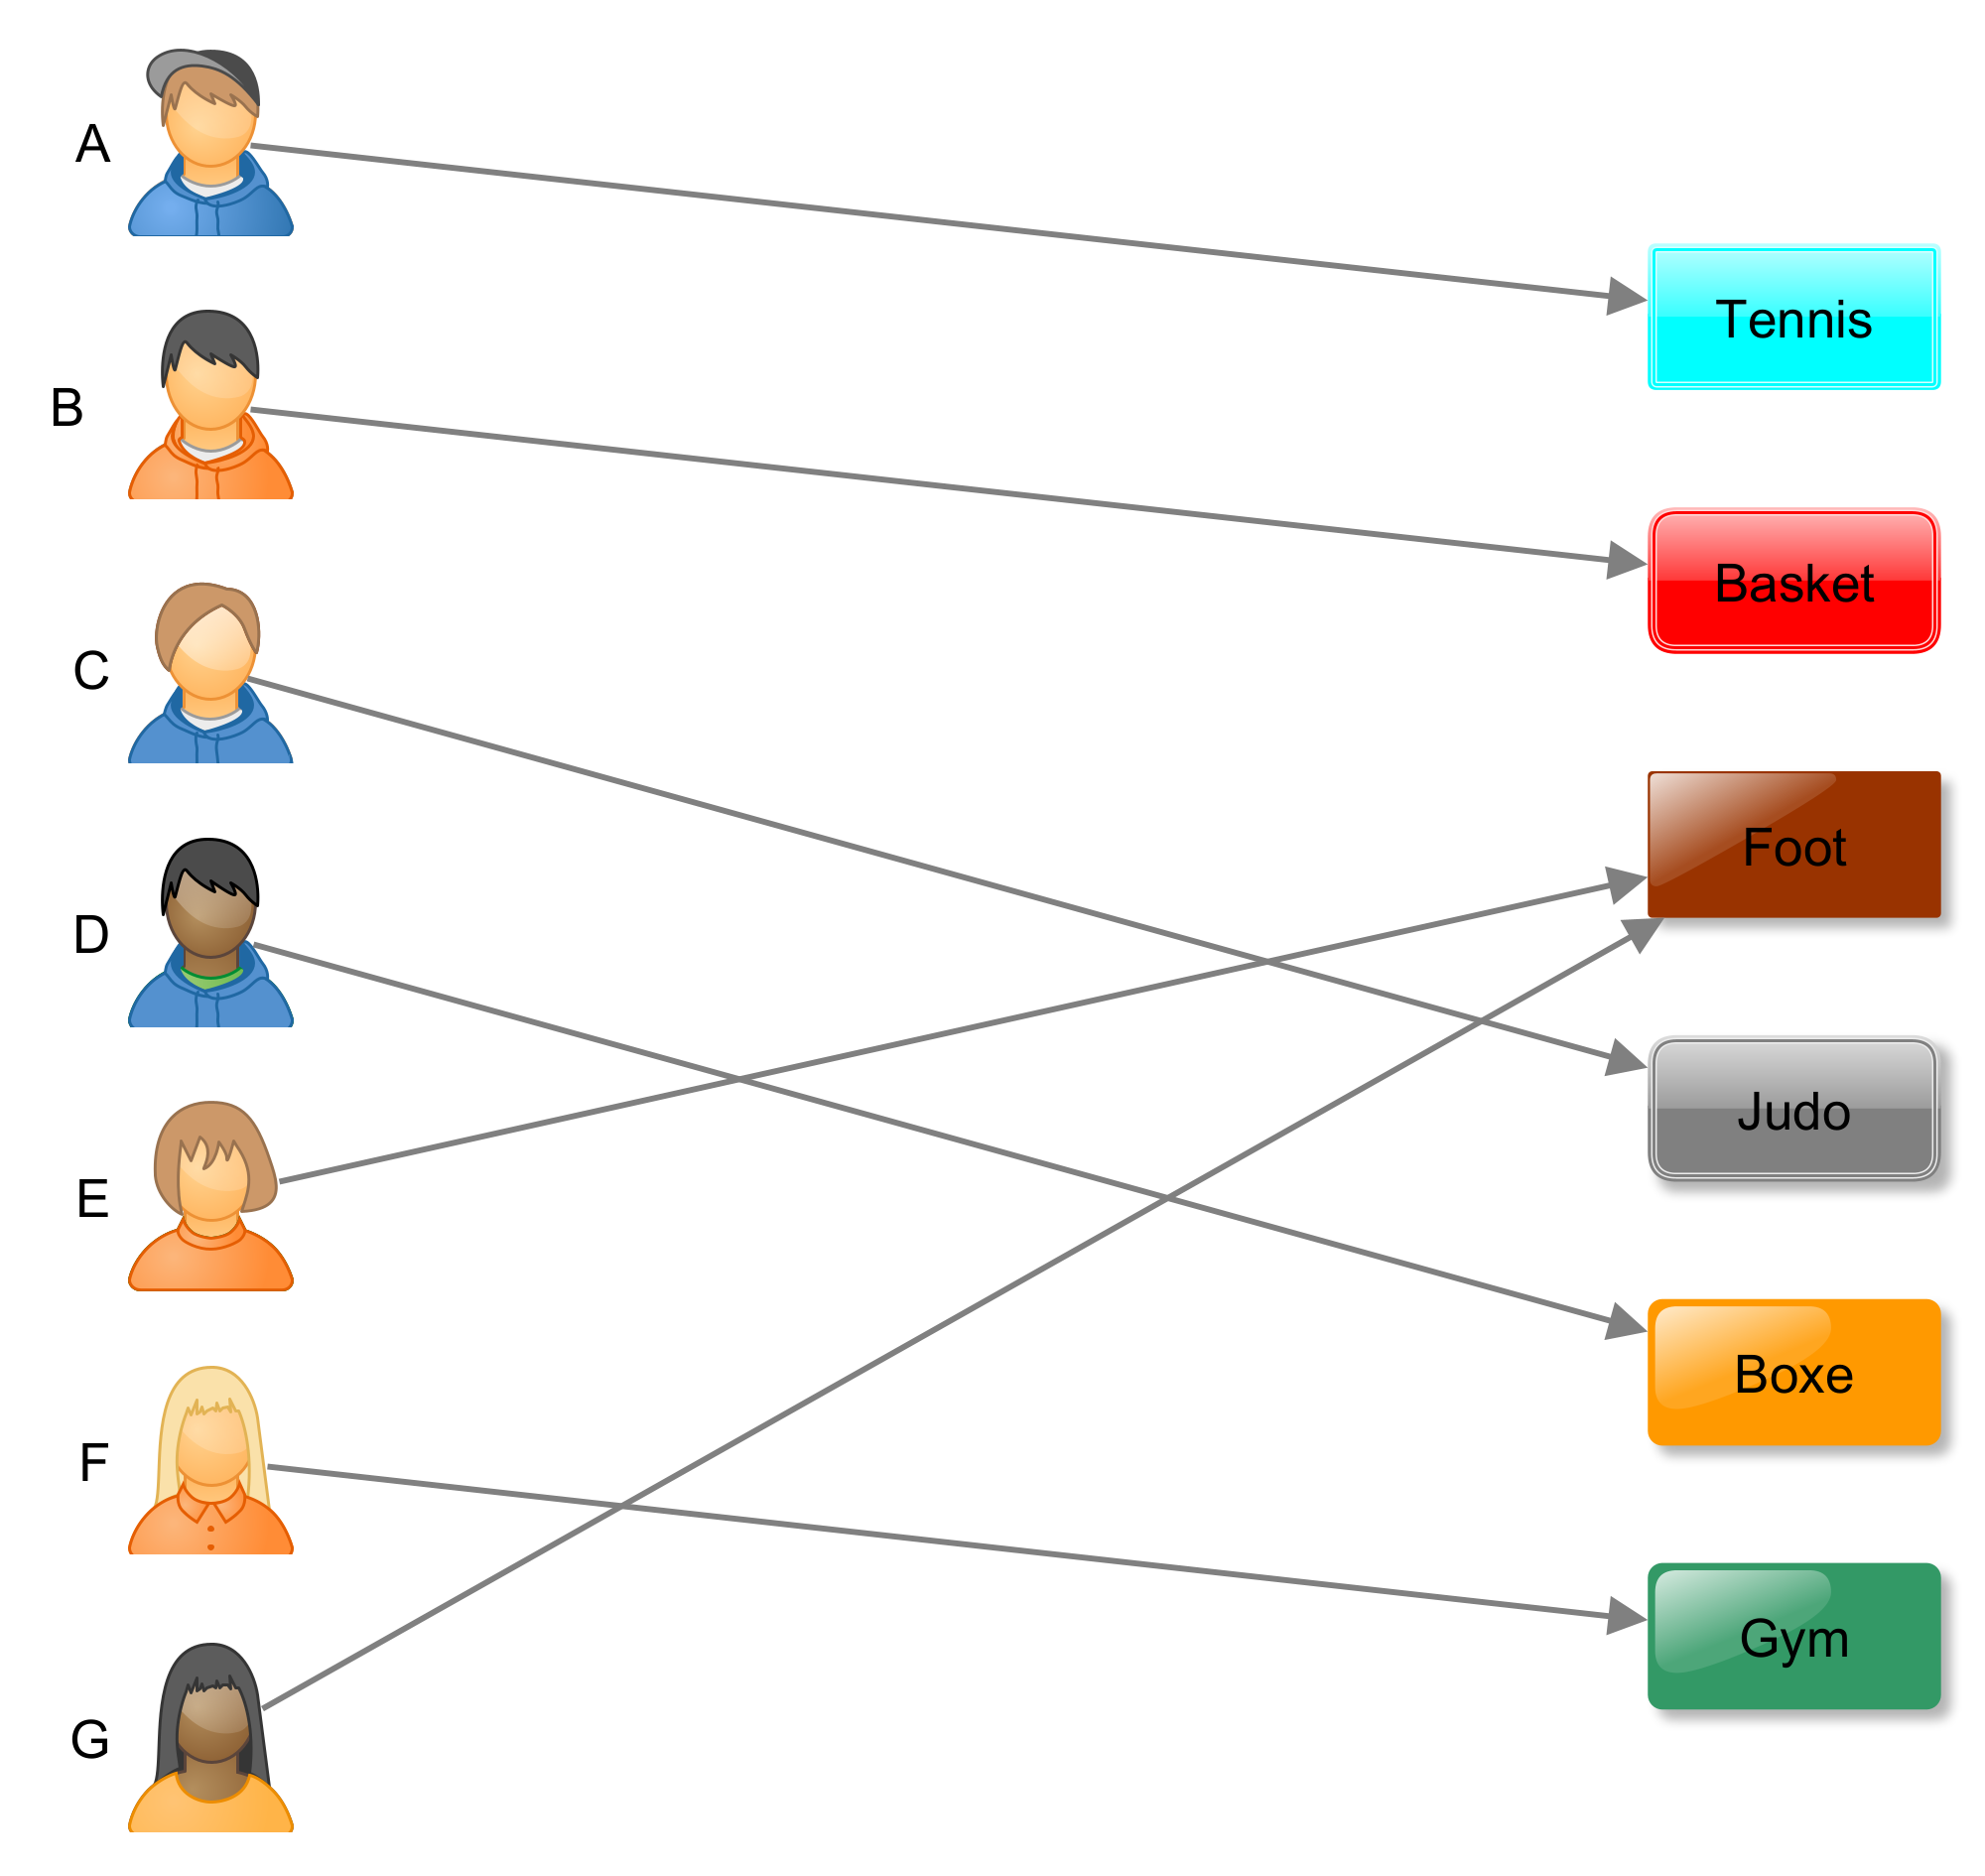
\includegraphics[height = 5cm]{img/dico_1}
\end{center}
Un sport peut être cité par \emph{plusieurs} jeunes.\\
En revanche, chaque jeune ne peut citer qu'\emph{un seul} sport.
\end{frame}
\begin{frame}[fragile]{Dictionnaire}
On pourrait utiliser une ou plusieurs listes pour représenter ces données mais il y a mieux : le \textit{dictionnaire}.\pause
\begin{center}
    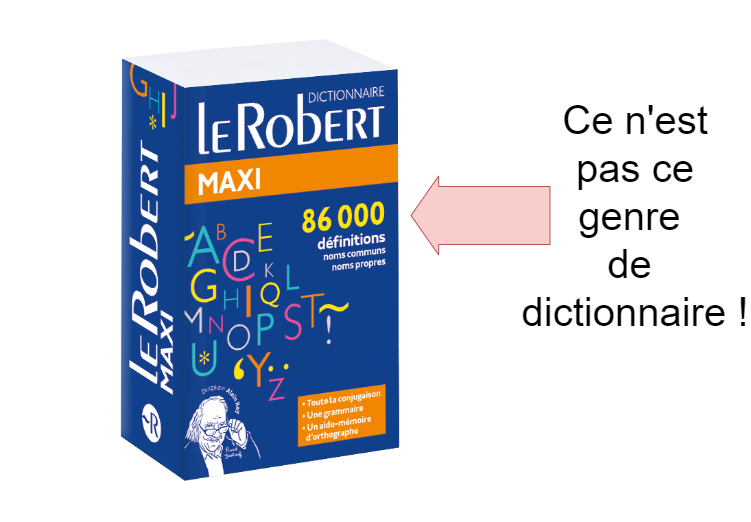
\includegraphics[height = 5cm]{img/dico_blague}
\end{center}
\end{frame}

\begin{frame}[fragile]{Un nouveau type}
La variable \pythoninline{sport} est de type \pythoninline{dict} :\pause
\begin{minted}{python}
sport = {'A' : 'Tennis', 'B' : 'Basket',
         'C' : 'Judo', ' D' : 'Boxe',
         'E' : 'Foot', 'F' : 'Gym',
         'G' : 'Foot'}
\end{minted}
\pause
La syntaxe générale est :

\pythoninline{variable = { cle1 : valeur1, cle2 : valeur2, ...}}
\end{frame}

\begin{frame}{Types autorisées}
\pythoninline{variable = { cle1 : valeur1, cle2 : valeur2, ...}}\\

\begin{enumerate}[--]
    \item 	Les valeurs peuvent être de n'importe quel type.\pause
    \item 	Les clés peuvent être \pause
    \begin{enumerate}[--]
        \item 	des \pythoninline{bool}, des \pythoninline{int}, des \pythoninline{float};\pause
        \item 	des \pythoninline{str}...\pause
        \item 	mais pas des \pythoninline{list} !
    \end{enumerate}
\end{enumerate}
On peut tout de même utiliser des \pythoninline{tuples} en guise de clés : \pause les \pythoninline{tuples} ressemblent aux \pythoninline{list} mais sont non modifiables.\\\pause

\pythoninline{a = (1, 2, 3)} est un exemple de \pythoninline{tuple}.
\end{frame}
\section{Opérations sur les dictionnaires}

\begin{frame}[fragile]{Accéder à une valeur par sa clé}
Pour connaître le sport préféré de \pythoninline{'A'}, c'est simple :\\\pause

\begin{minted}{python}
>>> sport['A']
'Tennis'
\end{minted}
\end{frame}

\begin{frame}{Créer de nouveaux couples \texttt{(clé / valeur)}}

Contrairement aux listes, il n'y a pas de méthode \texttt{append}.\\\pause
Pour intégrer l'information « le sport préféré de H est le Rugby » on écrira simplement :\\\pause

\pythoninline{sport['H']='Rugby'}
\end{frame}

\begin{frame}{Créer un dictionnaire vide et le peupler}

On peut partir d'un dictionnaire vide  \\\pause

\pythoninline{d = dict()}\\\pause

et remplir ses valeurs au fur et à mesure :

\pythoninline{d['bonjour'] = 'hello'}\\\pause

\pythoninline{d['crayon'] = 'pencil'}\\\pause

\pythoninline{d['se prélasser'] = 'to bask'}\\\pause

\textit{et c\ae tera}.
\end{frame}

\begin{frame}[fragile]{Parcourir l'ensemble des clés d'un dictionnaire}\pause
\begin{minted}{python}
for cle in d.keys():
    print(cle)
\end{minted}

\pause Ce script affiche \pause
\begin{minted}{python}
bonjour
crayon
se prélasser
\end{minted}
\end{frame}

\begin{frame}[fragile]{Parcourir l'ensemble des valeurs d'un dictionnaire}\pause
\begin{minted}{python}
for valeur in d.values():
    print(valeur)
\end{minted}

\pause Ce script affiche \pause
\begin{minted}{python}
hello
pencil
to bask
\end{minted}
\end{frame}

\begin{frame}[fragile]{Erreurs de clé}
\begin{minted}{python}
print(d['chien'])
\end{minted}

\pause Ce script produit une erreur : \pause

\color{red}\texttt{KeyError : 'chien'}
\end{frame}

\begin{frame}{Un exemple}
On veut créer un tableau de $10\times 10$ cases avec la valeur 0 dedans.\\\pause

On peut bien sûr créer cela avec une liste de listes (en compréhension).\\\pause

On peut utiliser un dictionnaire :\\\pause
\end{frame}
\begin{frame}[fragile]{Un exemple}

\begin{minted}[fontsize=\footnotesize]{python}
d = {(x, y) : 0 for x in range(1, 11) for y in range(1, 11)}
\end{minted}
\pause

\textbf{Avantages :}
\begin{itemize}
    \item 	plus simple à manipuler : on écrit \pythoninline{d[x, y]} au lieu de \pythoninline{d[x][y]} ;
    \item 	on n'est pas obligé de faire commencer les indices à zéro.
\end{itemize}

\textbf{Inconvénients :}
\begin{itemize}
    \item prend plus de place en mémoire (on s'en fiche un peu) ;
    \item plus flexible entraîne plus de possibilité d'erreurs !
\end{itemize}
\end{frame}


\section{Utilisation des dictionnaires}


\begin{frame}[fragile]{Données structurées}
Typiquement, pour stocker des données structurées :    \\\pause

\begin{minted}{python}
reseau = {'nom'        : 'local',
          'ip'         : '192.168.1.0',
          'masque'     : '255.255.255.0',
          'passerelle' : '192.168.1.254'}
\end{minted}
\end{frame}

\begin{frame}{Tables}

On utilise fréquemment des listes de dictionnaires...\\\pause

ou bien des dictionnaires de listes.
\end{frame}




\end{document}